\subsection{HDF5}
HDF5 is a data model , library and file format for storing and managing data. It defines an information set, which is a container of array variables, groups, and types. They are known as datasets, groups and datatype objects in HDF5 respectively. The data model defines mechanisms for creating associations between various information items. The main components of HDF5 are briefly described below.

File:
In the HDF5 data model the container of an HDF5 infoset
is represented by an HDF5 file. It is a collection of HDF5 objects and represents the relationship between them.
Every file begins with a root group "/", which serves as the "starting-point" in the object hierarchy. An empty file has atleast the root group in it.

Datasets:
HDF5 datasets are objects that represent actual data or content. Datasets are arrays which can have multiple dimensions. A dataset is characterized by a dataspace and a datatype. An HDF5 dataspace captures the rank (number of dimensions) , and the current and maximum extent in the respective dimensions. An HDF5 datatype describes the type of its data elements. 
HDF5 supports ten classes of datatypes including scalar types like integer, floating-point, string, etc. and compound datatypes. 

Groups:
HDF5 groups are akin to directories in a file system (reference here). A group is an explicit association between HDF5 objects. A group could contain multiple other groups, datasets or datatypes /textit{within} it. 
Traversing a root group generates the /information set graph/.

Attributes:
Aattributes are used for annotating datasets, groups, and datatype objects. They are datasets themselves, and are /textit{attached} to the existing objects they annotate. 

The above definitions are explained in the example shown in figure ~\ref{hdf5_example}. 
The file "sample.h5" contains a root group which itself contains a group G1 and two datasets, D1 and D2. Group G1 contains a dataset D3. Attribute A1 is linked to dataset D1. The datatype in all datasets in an integer. 

\begin{figure}[!t]
\centering
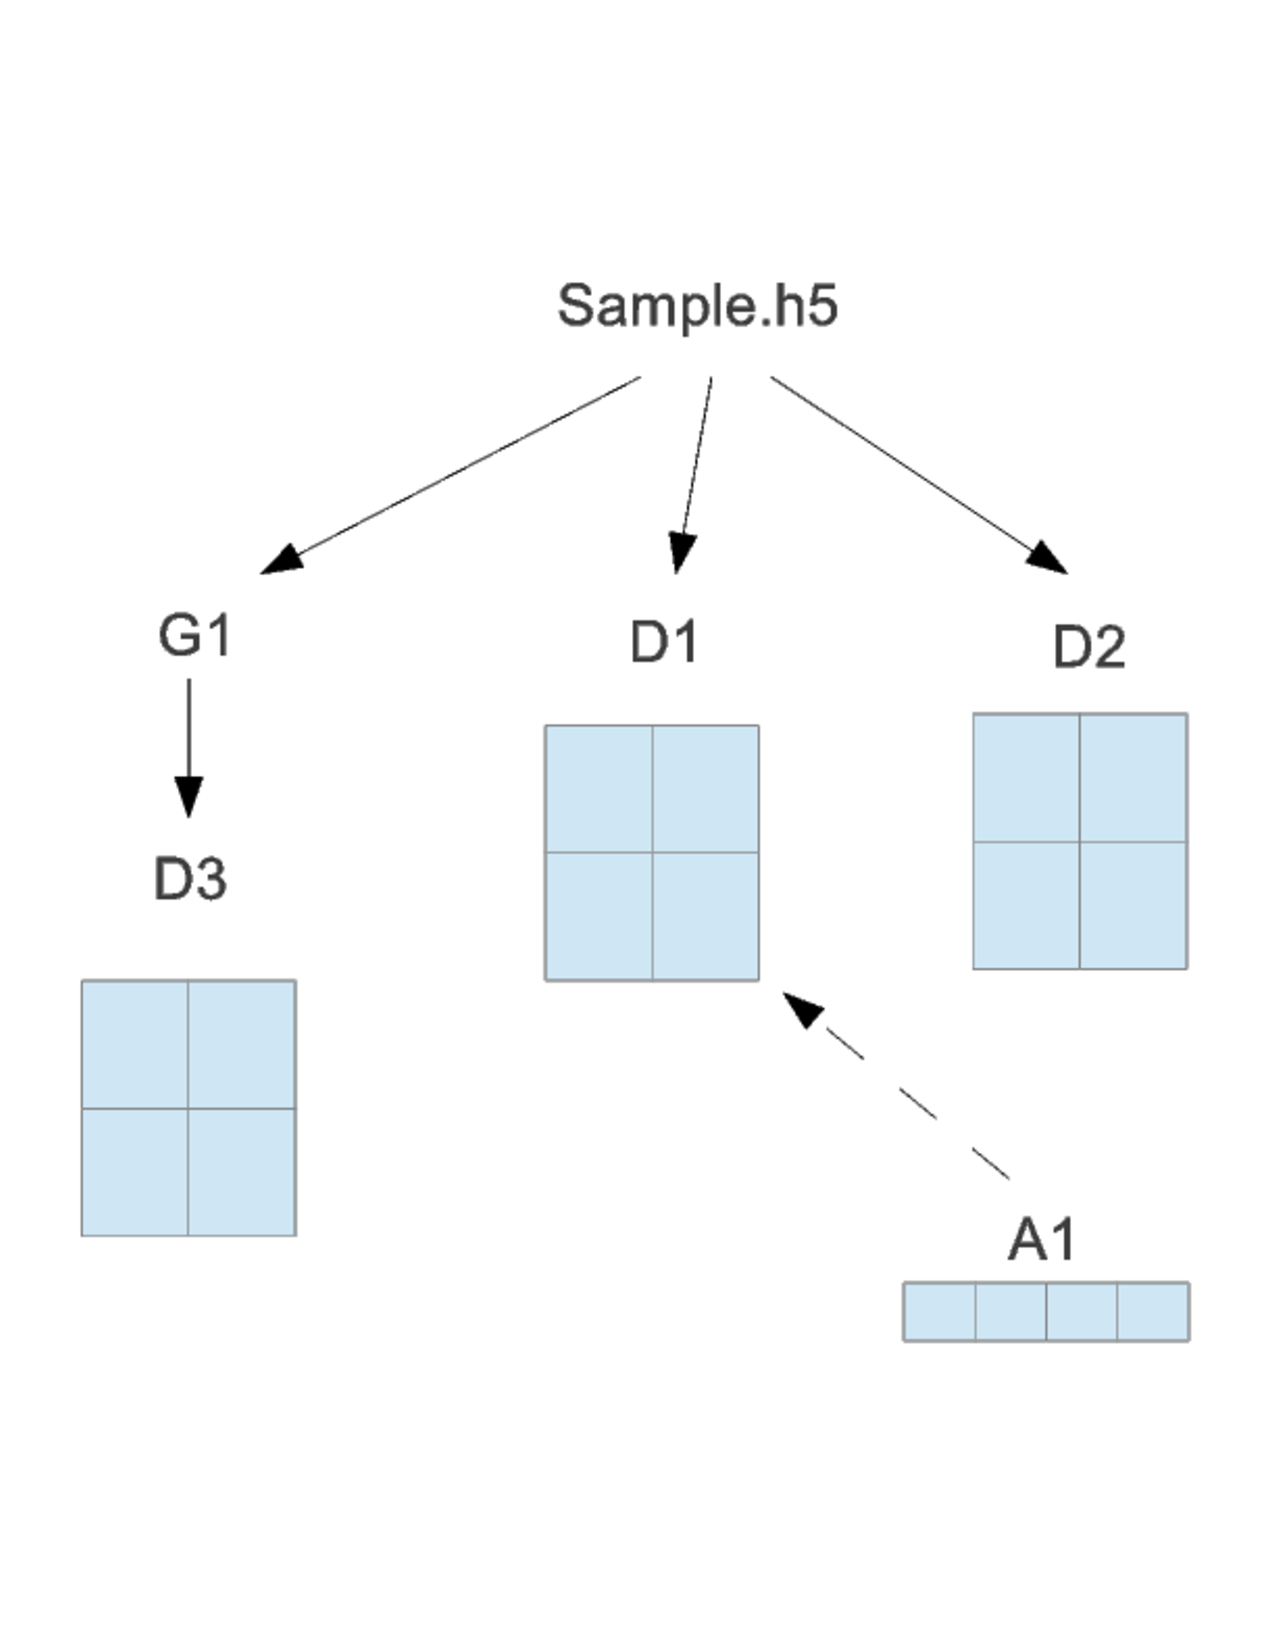
\includegraphics[width=2.5in]{hdf5_example}
\caption{A sample HDF5 file}
\label{hdf5_example}
\end{figure}

HDF5 file format:
An HDF5 file is a self-describing format which combines data and metadata. High level objects are stored alongwith metadata that is used to describe various characteristics about the object, alongwith the relationship between various objects.  

Parallel HDF5 (PHDF5):
As described previously, HDF5 supports parallelism using MPI. Multiple processes can be used to create and store objects in a file. PHDF5 exports a parallel I/O interface, where internally makes use of MPI-IO to perform I/O in parallel. 
Applications typically store multiple objects in a single HDF5 file. However, many popularly used parallel file systems like Lustre, Panasas etc. are known to perform poorly for workloads where multiple processes access a shared file (commonly referred to as the N-->1 access pattern). 

Virtual Object Layer (VOL):
(I have simply copied this part; need to reframe it) The Virtual Object Layer (VOL) is a new abstraction layer internal to the HDF5 library (reference here). It is implemented just below the public API. The VOL intercepts all HDF5 API calls that could potentially access objects in the file and forwards those calls to an “object driver” plugin. The plugins could actually store the objects in variety of ways. A plugin could, for example, have objects be distributed remotely over different platforms, provide a raw mapping of the model to the file system, or even store the data in other file formats (like native netCDF or HDF4 format). The user still gets the same data model where access is done to a single HDF5 “container”; however the plugin object driver translates from what the user sees to how the data is actually stored.

\subsection{PLFS}
PLFS is a middleware virtual file system that converts writes to a shared logical file into writes to multiple physical files. 
It is situated between the application and the parallel file system responsible for the actual data storage. 
It transforms an application's N-->1 access pattern into an N-->N access pattern, where every process participating in I/O writes data to its own , separate file. 
Thus, it interposes on application I/O and converts its I/O pattern into one that is more suitable for the underlying parallel file system.
The basic operation of PLFs is as follows. For every logical file, PLFS creates a /texit{container} structure on the underlying parallel file system. 
This container is a hierarchical directory tree consisting of multiple sub-directories. Multiple processes opening the same logical file for writing get a unique data file within the container. When the processes write to their file, a record identifying the write is appended to an index file shared between all processes. Thus, PLFS maintains sufficient metadata to recreate the shared logical file. A FUSE daemon exports this container structure as a single, logical file to the end-users, thereby keeping the PLFS operations transparent from them. 
We added a new feature to PLFS called XAttributes (xattrs). Xattrs serve as short metadata stored as key-value pairs.
All xattrs are stored in a new directory inside the PLFS container structure. They can be used to store user-defined information about data for easy and fast retrieval, since they are not stored alongwith raw data. 
We use xattrs to store metadata about HDF5 datasets. The datatype, number of dimensions and their extent etc. are stored as xattrs. 